% Classes of interpolation, integration and differentiation of CAP (src/core/Math/Interpolation, Integral, Derivative)
% and their dependencies. Used by the paper (section "Interpolation, integration and differentiation", figure
% fig:numerics) and by the Doxygen documentation (Integrator.hpp, Differentiation.hpp, Interpolation.hpp).
%   pdflatex NumericalTools.tex                                          -> NumericalTools.pdf (paper)
%   pdftoppm -r 200 -png -singlefile NumericalTools.pdf NumericalTools   -> NumericalTools.png (Doxygen)
%   pdftocairo -svg NumericalTools.pdf NumericalTools.svg                -> NumericalTools.svg
\documentclass[tikz,border=2pt]{standalone}
\usepackage[scaled=0.92]{helvet}
\usetikzlibrary{arrows.meta,shapes.multipart,positioning,fit,backgrounds}
\renewcommand{\familydefault}{\sfdefault}
\definecolor{abstract}{HTML}{D6E4F5}
\definecolor{concrete}{HTML}{EEF4FB}
\definecolor{steer}{HTML}{DCEFD9}
\definecolor{tools}{HTML}{FFF8E6}
\definecolor{dependline}{HTML}{8A6D3B}
\definecolor{folder}{HTML}{F7F7F7}
\begin{document}
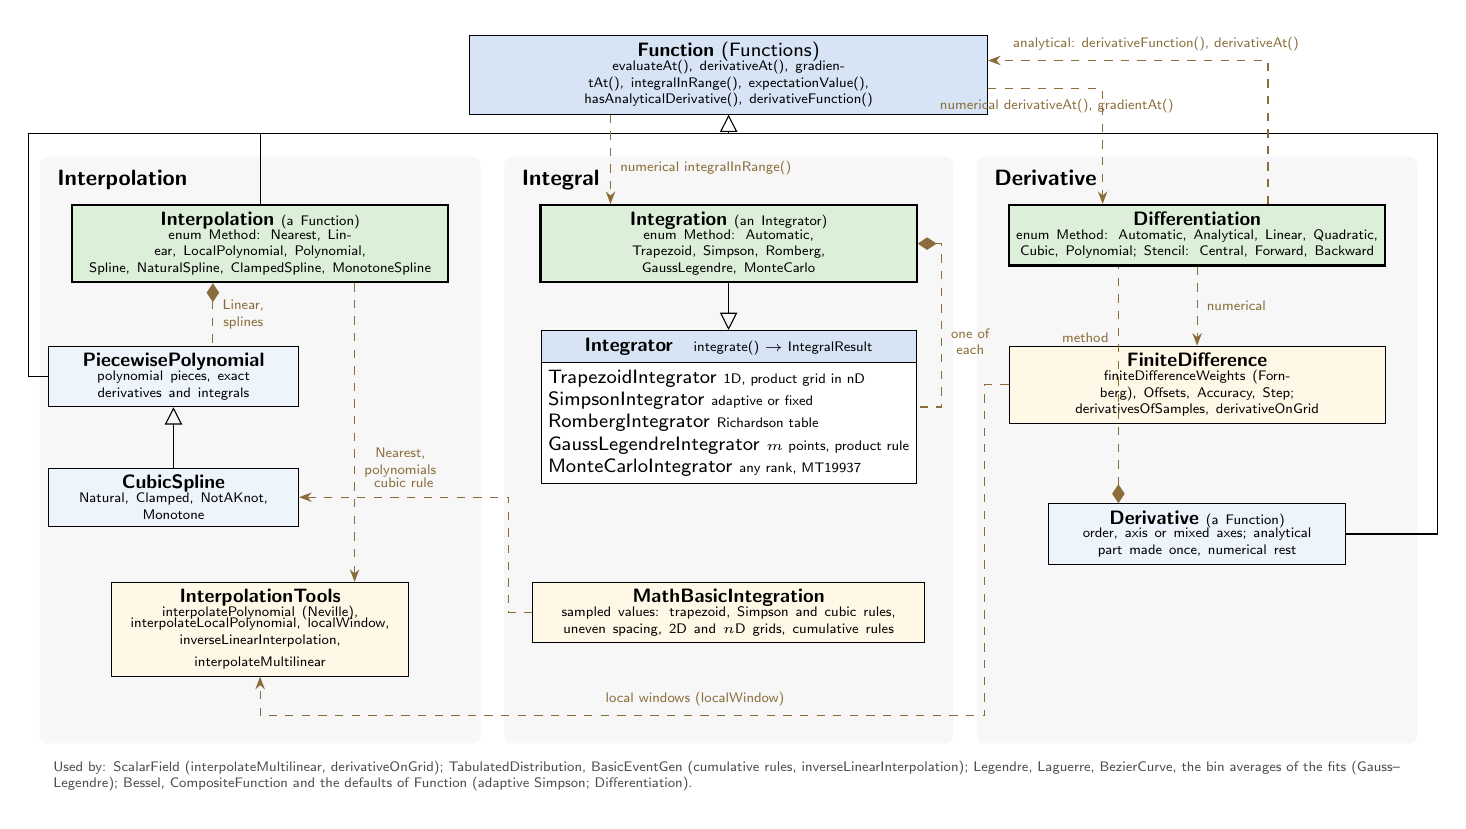
\begin{tikzpicture}[
    font=\scriptsize,
    cls/.style={draw, fill=concrete, align=center, inner sep=2.5pt, anchor=north, text width=#1},
    cls/.default=3.2cm,
    abs/.style={cls=#1, fill=abstract},
    abs/.default=3.2cm,
    steer/.style={cls=#1, fill=steer, line width=0.8pt},
    steer/.default=4.6cm,
    tool/.style={cls=#1, fill=tools},
    tool/.default=4.6cm,
    fam/.style={draw, rectangle split, rectangle split parts=2, rectangle split part fill={#1,white},
                rectangle split part align={center,left}, inner sep=2.5pt, anchor=north, align=left},
    inherit/.style={-{Triangle[open,length=2.2mm,width=2.2mm]}, thin},
    bus/.style={thin},
    uses/.style={dashed, dependline, -{Stealth[length=1.6mm]}, thin},
    owns/.style={dashed, dependline, {Diamond[length=2.4mm,width=1.6mm]}-, thin},
    lbl/.style={font=\tiny, text=dependline, align=center},
    title/.style={font=\footnotesize\bfseries, anchor=north west},
  ]

  % ---------------------------------------------------------------- folders
  \begin{scope}[on background layer]
    \fill[folder, rounded corners=3pt] (0.0,-1.15) rectangle (5.6,-8.6);
    \fill[folder, rounded corners=3pt] (5.9,-1.15) rectangle (11.6,-8.6);
    \fill[folder, rounded corners=3pt] (11.9,-1.15) rectangle (17.5,-8.6);
  \end{scope}
  \node[title] at (0.1,-1.2) {Interpolation};
  \node[title] at (6.0,-1.2) {Integral};
  \node[title] at (12.0,-1.2) {Derivative};

  % ---------------------------------------------------------------- Function
  \node[abs=6.4cm] (Function) at (8.75,0.4)
    {\textbf{\textit{Function}} (Functions)\\[-1pt]
     \tiny evaluateAt(), derivativeAt(), gradientAt(), integralInRange(), expectationValue(),\\[-2pt]
     \tiny hasAnalyticalDerivative(), derivativeFunction()};

  % ---------------------------------------------------------------- Interpolation
  \node[steer] (Interpolation) at (2.8,-1.75)
    {\textbf{Interpolation} \tiny(a Function)\\[-1pt]
     \tiny enum Method: Nearest, Linear, LocalPolynomial, Polynomial,\\[-2pt]
     \tiny Spline, NaturalSpline, ClampedSpline, MonotoneSpline};
  \node[cls=3.0cm] (Piecewise) at (1.7,-3.55)
    {\textbf{PiecewisePolynomial}\\[-1pt]\tiny polynomial pieces, exact\\[-2pt]\tiny derivatives and integrals};
  \node[cls=3.0cm] (Spline) at (1.7,-5.1)
    {\textbf{CubicSpline}\\[-1pt]\tiny Natural, Clamped, NotAKnot,\\[-2pt]\tiny Monotone};
  \node[tool=3.6cm] (InterpTools) at (2.8,-6.55)
    {\textbf{InterpolationTools}\\[-1pt]
     \tiny interpolatePolynomial (Neville),\\[-2pt]\tiny interpolateLocalPolynomial, localWindow,\\[-2pt]
     \tiny inverseLinearInterpolation, interpolateMultilinear};
  \draw[inherit] (Spline.north) -- (Piecewise.south);
  \draw[owns] ([xshift=-0.6cm]Interpolation.south) -- node[lbl, right]{Linear,\\splines} ([xshift=0.5cm]Piecewise.north);
  \draw[uses] ([xshift=1.2cm]Interpolation.south) -- node[lbl, right, pos=0.6]{Nearest,\\polynomials} ([xshift=1.2cm]InterpTools.north);

  % ---------------------------------------------------------------- Integral
  \node[steer] (Integration) at (8.75,-1.75)
    {\textbf{Integration} \tiny(an Integrator)\\[-1pt]
     \tiny enum Method: Automatic, Trapezoid, Simpson, Romberg,\\[-2pt]
     \tiny GaussLegendre, MonteCarlo};
  \node[fam=abstract] (Integrator) at (8.75,-3.35)
    {\textbf{\textit{Integrator}}\quad\tiny integrate() $\to$ IntegralResult\nodepart{two}%
     TrapezoidIntegrator \tiny 1D, product grid in nD\\
     SimpsonIntegrator \tiny adaptive or fixed\\
     RombergIntegrator \tiny Richardson table\\
     GaussLegendreIntegrator \tiny $m$ points, product rule\\
     MonteCarloIntegrator \tiny any rank, MT19937};
  \node[tool=4.8cm] (Sampled) at (8.75,-6.55)
    {\textbf{MathBasicIntegration}\\[-1pt]
     \tiny sampled values: trapezoid, Simpson and cubic rules,\\[-2pt]
     \tiny uneven spacing, 2D and $n$D grids, cumulative rules};
  \draw[inherit] (Integration.south) -- (Integrator.north);
  \draw[owns] (Integration.east) -- ++(0.3,0) |- node[lbl, right, pos=0.3]{one of\\each} (Integrator.east);
  \draw[uses] (Sampled.west) -- ++(-0.3,0) |- node[lbl, above, pos=0.75]{cubic rule} (Spline.east);

  % ---------------------------------------------------------------- Derivative
  \node[steer] (Differentiation) at (14.7,-1.75)
    {\textbf{Differentiation}\\[-1pt]
     \tiny enum Method: Automatic, Analytical, Linear, Quadratic,\\[-2pt]
     \tiny Cubic, Polynomial; Stencil: Central, Forward, Backward};
  \node[tool=4.6cm] (FD) at (14.7,-3.55)
    {\textbf{FiniteDifference}\\[-1pt]
     \tiny finiteDifferenceWeights (Fornberg), Offsets, Accuracy, Step;\\[-2pt]
     \tiny derivativesOfSamples, derivativeOnGrid};
  \node[cls=3.6cm] (Derivative) at (14.7,-5.55)
    {\textbf{Derivative} \tiny(a Function)\\[-1pt]\tiny order, axis or mixed axes; analytical\\[-2pt]\tiny part made once, numerical rest};
  \draw[uses] (Differentiation.south) -- node[lbl, right]{numerical} (FD.north);
  \draw[owns] ([xshift=-1.0cm]Derivative.north) -- node[lbl, left, pos=0.7]{method} ([xshift=-1.0cm]Differentiation.south);
  \draw[uses] (FD.west) -- ++(-0.3,0) |- node[lbl, above, pos=0.7]{local windows (localWindow)} (2.8,-8.25) -- (InterpTools.south);

  % ---------------------------------------------------------------- inheritance from Function
  \draw[bus] (Interpolation.north) -- (Interpolation.north |- 0,-0.85) -- (17.75,-0.85) |- (Derivative.east);
  \draw[bus] (Piecewise.west) -- ++(-0.25,0) |- (Interpolation.north |- 0,-0.85);
  \draw[inherit] (Function.south |- 0,-0.85) -- (Function.south);

  % ---------------------------------------------------------------- the defaults of Function and the analytical derivatives
  \draw[uses] ([xshift=-1.5cm]Function.south) -- node[lbl, right, pos=0.6]{numerical integralInRange()} ([xshift=-1.5cm]Integration.north);
  \draw[uses] ([yshift=-0.18cm]Function.east) -| node[lbl, below, pos=0.3]{numerical derivativeAt(), gradientAt()} ([xshift=-1.2cm]Differentiation.north);
  \draw[uses] ([xshift=0.9cm]Differentiation.north) |- node[lbl, above, pos=0.7]{analytical: derivativeFunction(), derivativeAt()} ([yshift=0.18cm]Function.east);

  % ---------------------------------------------------------------- users
  \node[font=\tiny, text=gray!60!black, align=left, anchor=north west, text width=17.3cm] at (0.05,-8.7)
    {Used by: ScalarField (interpolateMultilinear, derivativeOnGrid); TabulatedDistribution, BasicEventGen (cumulative
     rules, inverseLinearInterpolation); Legendre, Laguerre, BezierCurve, the bin averages of the fits (Gauss--Legendre);
     Bessel, CompositeFunction and the defaults of Function (adaptive Simpson; Differentiation).};
\end{tikzpicture}
\end{document}
